%%%%%%%%%%%%%%%%%%%%%%%%%%%%%%%%%%%%%%%%%%%%%%%%%%%%%%%%%%%%%%%%%%%%%%%%%%%%%%
\section {Data Quality Monitoring - DQM}

\begin{itemize}
\item 
  DQM jobs are standalone art jobs which connect to the artdaq dispatcher and request events.
  We envisage one DQM job per detector subsystem.
\item
  FHICL files of the DQM jobs are stored in the same subdirectory with other FHICL files -
  \$config\_dir/\$config\_name. 
\item
  DQM jobs are started by the {\bf mu2e\_config} frontend at begin run.
\item
  the DAQ jobs use ROOT v6.32.08+ built with +http7+webgui options and rely on THttpServer/RBrowser 
  to publish the histograms.
\item
  In principle, only one port per subsystem is needed. The used values need to be coordinated.
  An example of the DQM port assignment:
  \begin{itemize}
  \item 
    tracker:8877, calorimeter: 8867. CRV: 8857, STM: 8847, EXM: 8837, DAQ (if needed): 8827. 
  \end{itemize}
\end{itemize}

An example of the DQM configuration section is shown in Figure 
\begin{figure}[H]
  \begin{tikzpicture}
    \node[anchor=south west,inner sep=0] at (0,0.) {
      % \node[shift={(0 cm,0.cm)},inner sep=0,rotate={90}] at (0,0) {}
      \makebox[\textwidth][c] {
        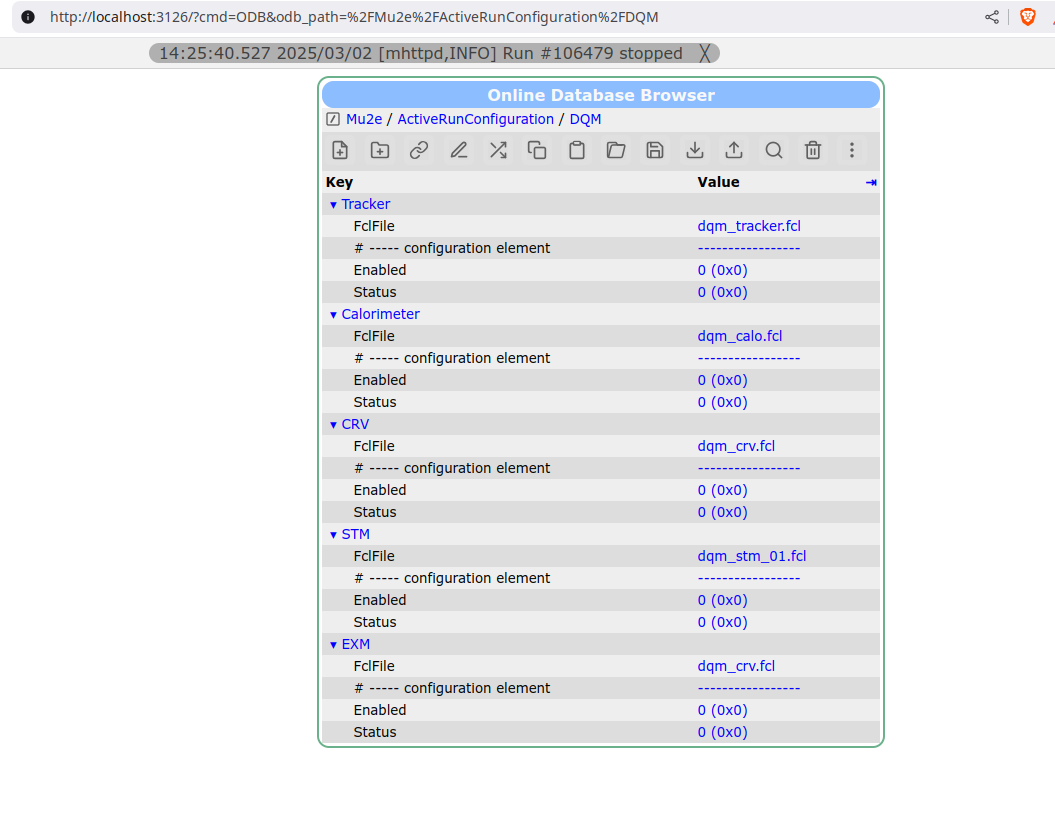
\includegraphics[width=0.95\textwidth]{png/dqm_configuration}
      }
    };
    % \node [text width=8cm, scale=1.0] at (14.5,0.5) {$\mu_B$, expected background mean};
    % \node [text width=8cm, scale=1.0, rotate={90}] at (1.5,7.5) { $S_{D}$, ``discovery'' signal strength  };
  \end{tikzpicture}
  \caption{
    \label{figure:dqm_configuration}
    DQM configuration
  }
\end{figure}



%%% Local Variables:
%%% mode: latex
%%% TeX-master: t
%%% End:
